\subsection{Contrastive Learning}
The method proposed by \citet{shenkar2022anomaly} utilizes an internal contrastive learning algorithm, termed InterCont, for tabular data. 
This represents a novel application of contrastive learning, a field that has primarily received attention within the domains of computer vision and natural language processing. 
The fundamental objective of such a network is to differentiate between distinct instances, such as distinguishing an image of a cat from images of other animals. 
To achieve this, the network must extract discriminative features from the input data. \todo{explain why this is representation learning, citing the chapter befor}


This chapter establishes a framework for analyzing contrastive learning algorithms by detailing their core components. 
Although various approaches to constructing contrastive learning networks exist, the primary architecture has converged toward a stable structural standard \citep[6]{hu2021survey}. 
The subsequent sections outline this framework, beginning with data augmentation strategies, using computer vision as a primary example. 
This is followed by an explanation of the conventional network structure, which typically comprises an encoder network, a projection head, and occasionally a prediction head. 
The chapter concludes with an examination of the most prominent contrastive loss functions.


\subsection*{Data Augmentation}
\begin{figure}[H]
    \centering
    \begin{minipage}{0.35\textwidth}
        \onehalfspacing
        The model is provided with an anchor, which represents a specific data instance, such as an image, that serves as the reference point for differentiation. 
        A positive sample is generated by applying random data augmentation techniques to this anchor. 
        In the context of computer vision, common augmentation strategies include cropping, flipping, and rotating. 
        Since the anchor and the positive sample originate from the same source, the objective is for the model to map them to proximal positions within the feature space. 
    \end{minipage}%
    \hfill 
    \begin{minipage}{0.6\textwidth}
        \centering
        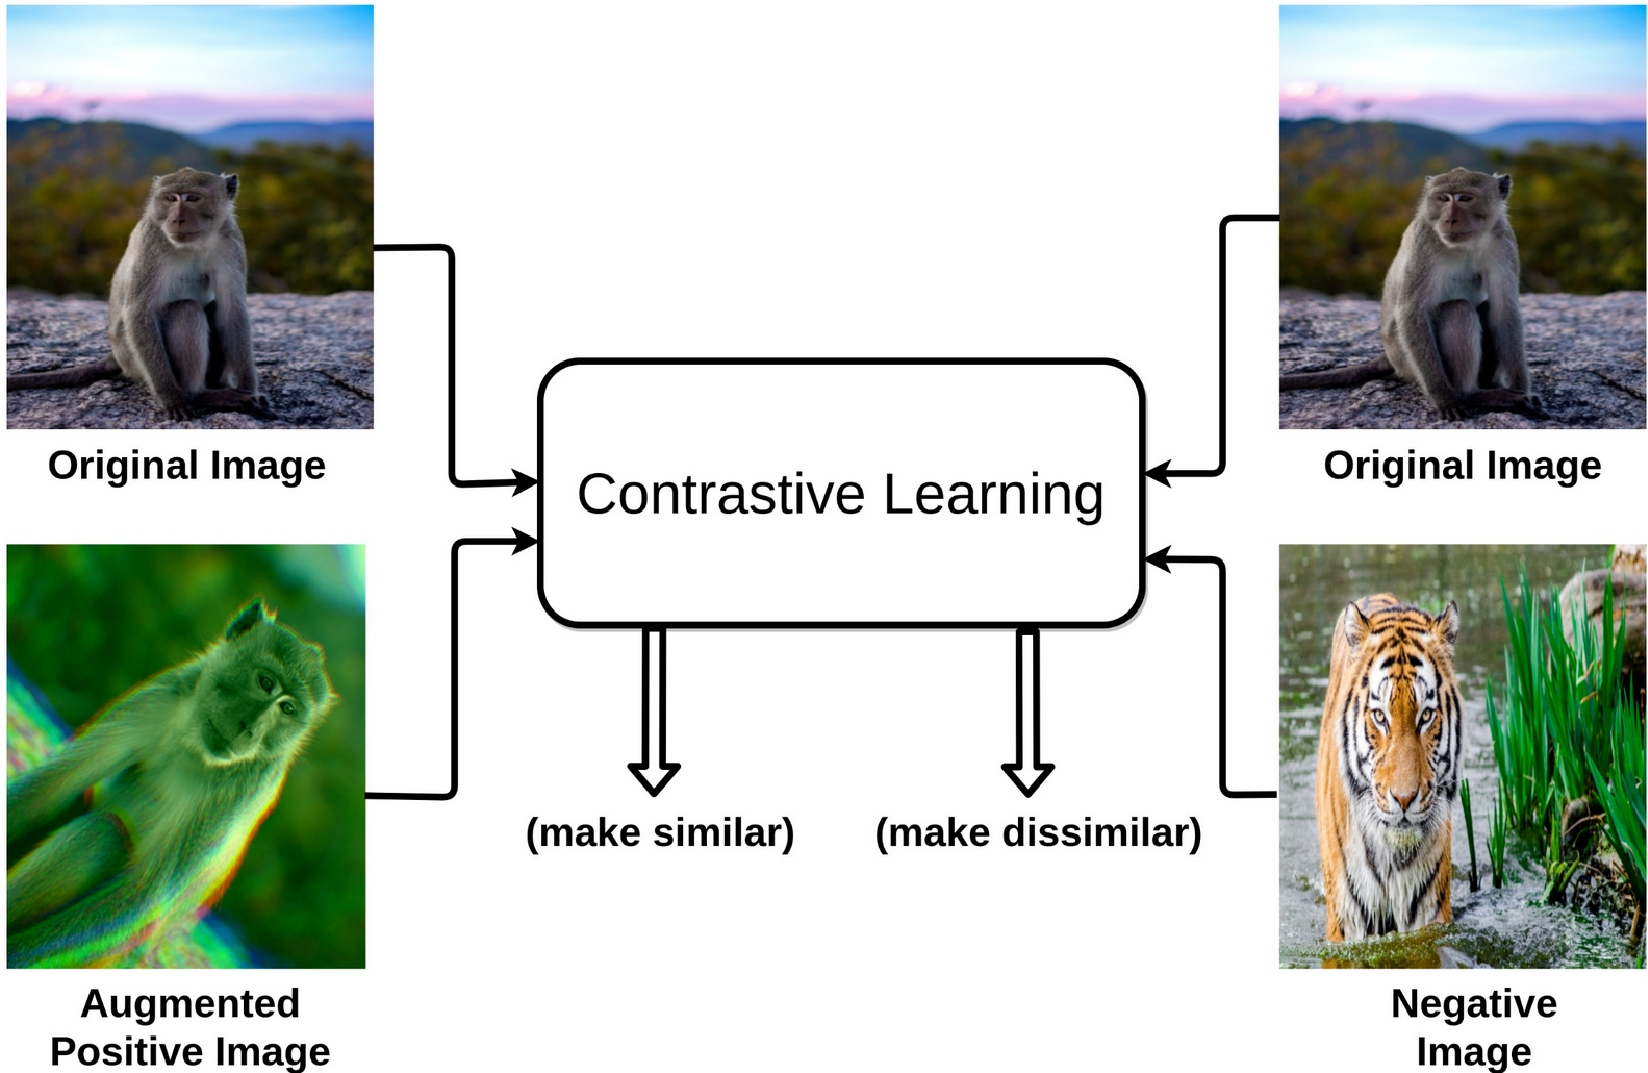
\includegraphics[width=\textwidth]{Images/Contrastive_learning_intuition}
        \caption{Intuition behind Contrastive Learning}
    \end{minipage}
    \label{fig:contrastive_intuition}
\end{figure}

Various methodologies exist for data augmentation; for an extensive overview of these techniques within contrastive learning, see \citet{chen2020simple}.
Conversely, a negative pair consists of the anchor and a distinct data instance, referred to as the negative sample. 
The optimization goal is to maximize the distance between the anchor and negative samples in the feature space relative to the distance between the anchor and positive samples. 
Selecting appropriate negative samples remains a significant challenge, as they must be sufficiently informative to provide the necessary signal for the network to learn diverse and robust representations. 
Hard negatives, which are semantically similar and lie close to the anchor in the feature space, are particularly valuable for this process \citep{jang2021adversarial}. 
By training on a diverse set of such samples, the model enhances its ability to identify the subtle features that distinguish different objects. 
This mechanism mitigates the risk of overfitting and reduces the impact of data biases, thereby improving the generalization performance of the model.\todo{why?} 
However, simply incorporating an arbitrary number of random instances often fails to provide the required hard negatives. 
It is therefore essential to consider the specific characteristics of the task and the dataset when curating negative samples to minimize the influence of misleading or uninformative data.
\todo{most important bc ICL does this with internal data - but subject to next chapter}
\todo{add: Methods of sampling negatives} 
\todo{add: Sliding window other papers that use that}
\todo{add: Sliding Window: critizms: geometric Concentration, syntax vs semantics trade off, selection bias and false negatives}
\todo{insert solution for sample selection to critize InterCont}


\subsubsection*{Network Structure}
The encoder network accepts augmented data instances as input and embeds them into a latent space designed to capture meaningful features and semantic similarities. 
This latent space represents an abstract, compressed, and low-dimensional vector space where essential patterns of the input data are encoded while filtering out noise and redundant information. 
The architecture typically utilizes a bottleneck design, characterized by hidden layers with fewer nodes than the preceding layers, which enforces the necessary data compression.
In the context of autoencoders, the system consists of two primary components: the encoder, which maps high-dimensional input to a reduced vector, and the decoder, which attempts to reconstruct the original input from this compressed representation. 
The network is trained to minimize the reconstruction error, ensuring the encoder retains only the most critical information.


\begin{figure}[htbp]   
    \centering
    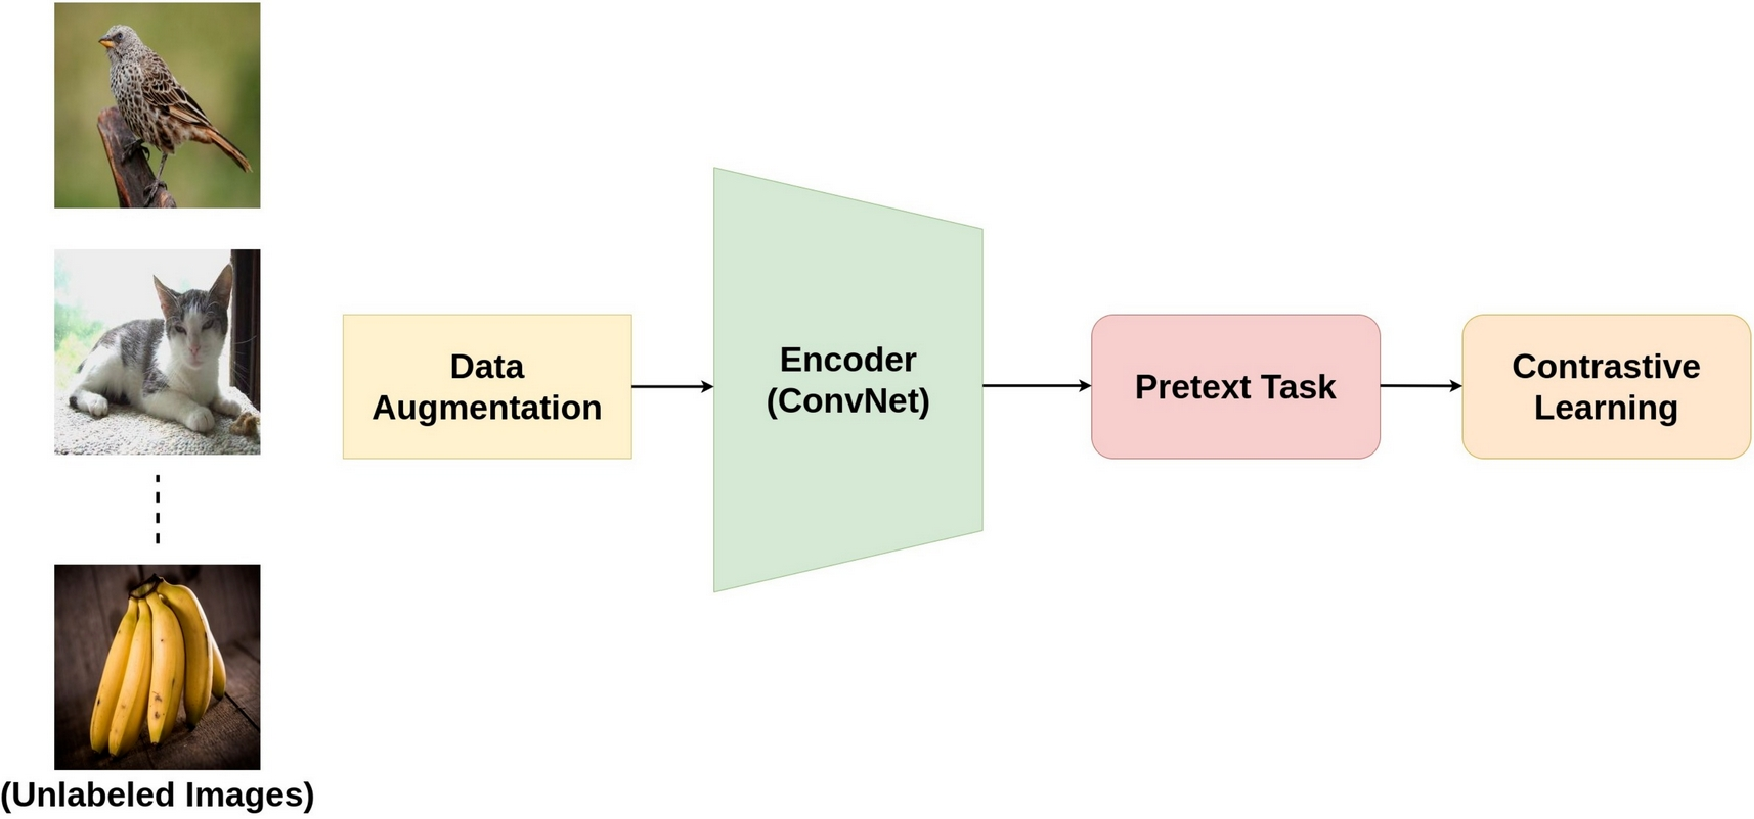
\includegraphics[width=0.6\textwidth]{Images/contrastive_learning_pipeline.pdf}
    \caption{Contrastive Learning pipeline}
    \label{fig:pipeline}
\end{figure}


Following the encoding process, the resulting representation is passed to a projection head. \todo{insert image}
This component is a non-linear neural network layer, often implemented as a multi-layer perceptron (MLP) \todo{what?}, which further refines the learned representations by mapping them to a space where the contrastive loss is applied.\todo{whats the reason to put it in? how does it work? - ICL is missing this!} 
This refinement is a standard practice in modern contrastive learning frameworks to improve the quality of the downstream features. 
Furthermore, certain architectures, such as Bootstrap Your Own Latent (BYOL) \todo{right name?} \citep{grill2020bootstrap}, incorporate an additional non-linear prediction head. 
This extra layer is used to predict the representation of one view from another, further enhancing the robustness and discriminative power of the algorithm. \todo{explain in more detail}
Some frameworks \todo{example} also implement a momentum encoder, which maintains a slowly evolving version of the network weights to ensure consistency in the representation space across training iterations.


\subsubsection*{Contrastive loss function}
The contrastive loss function pursues an objective distinct from the loss functions discussed in Chapter two. 
Its primary purpose is to minimize the distance between the anchor and positive samples in the feature space while simultaneously maximizing the distance between the anchor and negative samples. 
The selection of a specific loss function is contingent upon the network architecture and the inherent characteristics of the dataset. 
The most widely adopted contrastive loss function is Information Noise-Contrastive Estimation (InfoNCE). 
In practical applications, modified versions of this objective are frequently implemented to suit specific requirements. 
For a comprehensive overview of various contrastive loss functions, see \citet{le2020contrastive}. This thesis focuses specifically on InfoNCE, as it is the loss function utilized in the methodology proposed by \citet{shenkar2022anomaly}.


\textbf{Info noise-contrastive estimation (InfoNCE)} represents an optimized iteration of the Noise-Contrastive Estimation (NCE) originally proposed by \citet{gutmann2010noise}. Formulated by \citet{oord2018representation}, the function incorporates principles of mutual information \todo{define in a own passage} to enhance representation learning. 
The objective of InfoNCE is to maximize the lower bound of the mutual information between positive pairs while minimizing the mutual information between negative pairs. 
By treating the contrastive task as a multi-class classification problem where the model must identify the single positive sample among a set of noise samples, the function effectively guides the encoder to learn high-dimensional features. \todo{what?}
It is defined as:

\begin{equation}
    \mathcal{L}_{N} = -\mathbb{E}_{X} \left[ \log \frac{f_k(x_{t+k}, c_t)}{\sum_{x_j \in X} f_k(x_j, c_t)} \right] .
\end{equation}

In this formulation, $x_t+k$ represents the positive samples, while $x_j$ denotes the negative samples. 
The term $f_k$ serves as the density ratio, quantifying the alignment between the pairs, and $N$ acts as a scaling factor that influences the difficulty of the task by regulating the amount of information considered. 
The equation calculates an expectation across the dataset, utilizing a logarithmic transformation to manage the exponential growth of the similarity scores. 
The primary objective is to maximize the probability of correctly identifying the positive sample from the set. 
By applying a negative sign to the expectation, the loss function is minimized.
Consequently, if the probability of selecting the correct sample is 1, the resulting loss becomes 0.


The loss function facilitates the maximization of mutual information, which quantifies the statistical dependence between two variables. \todo{own passage write it above}
Specifically, mutual information measures the reduction in uncertainty regarding one variable given knowledge of another. 
By minimizing the InfoNCE loss, it is mathematically demonstrated that the lower bound of the mutual information between the original data and its latent representation is maximized. 
Consequently, the learned representation captures the most significant features of the input data, effectively preserving its essential characteristics. \todo{more details}
For a rigorous mathematical proof of this relationship, see \citet{oord2018representation}. This derivation further indicates that the lower bound of the mutual information is constrained by the number of negative samples utilized during training. 
Specifically, the capacity of the model to capture information increases as a function of the number of negative samples, as a larger set of negatives provides a more challenging and precise contrast for the anchor. 
This relationship suggests that increasing the quantity of negative samples directly enhances the information density of the resulting representations.\todo{source}


\subsubsection*{Alternative Contrastive Loss functions}
Cross-entropy loss quantifies the divergence between the predicted probability distribution and the actual distribution of a variable, a metric frequently utilized in classification tasks. 
Within the framework of contrastive learning, the training data is typically partitioned into batches to facilitate the calculation of this loss. 
In this context, the task is reframed as a multi-class classification problem where, for a given anchor, the model must correctly identify its corresponding positive sample from a set of candidates within the batch. 
The cross-entropy loss is defined as follows: \todo{is that passage needed?}


